\subsection{Znaczenie szkieletów aplikacji}
	Internetowe szkielety aplikacji nie są same w sobie bibliotekami programistycznymi. Stanowią one raczej ich zbiór, jak również zestaw narzędzi, mających na celu ułatwienie programiście implementacji własnego rozwiązania. Bardzo często są one również praktyczną implementacją standardów (tak jak \textbf{Seam Framework}) i tak zwanych \textbf{best practices}. Jest to szczególnie użyteczne ponieważ nierzadko zdarza się, że programista popełnia błąd na pewnym etapie projektowanie lub implementacji określonego modułu, którego późniejsze konsekwencje wymagają stworzenia niepotrzebnego i nadmiarowego kodu, czego dałoby by się uniknąć, gdyby podążano już wyznaczonymi ścieżkami. Prawdziwe w takim wypadku staje się również zdanie, że jeden błąd generuje kolejne, a te mogą być zalążkiem następnych.
	
	Powodem istnienia szkieletów aplikacji jest więc zapobieganie takim sytuacjom, poprzez proponowanie już gotowych modułów, które są przetestowane i ciągle modyfikowane przez doświadczone osoby, celem dostarczenia jeszcze lepszych rozwiązań \cite{art_of_java_web_dev}.
	
	Oprogramowanie zorientowane obiektowo jest doskonałym zobrazowaniem koncepcji wykorzystania szkieletu jako fundamentu do budowy własnego rozwiązania. Na najniższym poziomie szczegółowości każdy program czy też moduł większej części, jest zbiorem klas posiadającym jasno określony zbiór ról - obowiązków, a których obiekty współpracują ze sobą, celem dostarczenia gotowego wyniku lub jego części. Wspólnie te obiekty reprezentują pewną koncepcję, dla realizacji której zostały utworzone. 
	
	W kontekście szkieletu aplikacji internetowych można więc wyróżnić klasy przeznaczone do kooperacji z bazą danych, odpowiedzialnych za walidację informacji czy też pomocnych w momencie renderowania widoku. Warto nadmienić, że te zasady są równie ważne dla małych systemów, jak i dla dużych. Niemniej, w pierwszym przypadku, gdzie poziom skomplikowania jest niski, nie ma potrzeby definiowania wielu poziomów abstrakcji ułatwiających określone czynności, jak na przykład wcześniej wymienione walidacje danych. Niestety z czasem, początkowo prosty system, staje się coraz bardziej skomplikowany i bardzo często programista nie jest już wtedy w stanie zapanować na chaosem oraz dostarczyć zunifikowanego sposobu rozwiązywania powtarzalnych czynności. Z tego powodu dobry szkielet programistyczny charakteryzuje się jasno, ale nie sztywno zdefiniowanymi granicami między poszczególnymi zbiorami funkcjonalnymi. Wprowadzone poziomy abstrakcji, często więcej niż jeden dla pojedynczego celu, jak na przykład sposób interakcji systemu i jego klientów, są wynikiem wieloletnich zmian, podczas których zidentyfikowano wiele wspólnych problemów i dla których znaleziono rozwiązanie w postaci ram projektowych czy też \textbf{best pratices}, będących ostatecznie właściwą esencją znaczenia szkieletu aplikacji \cite{framework_design_-_a_role_modeling_approach}.
	
	Dobrymi przykładami tutaj będą z pewnością warstwy abstrakcji dla obsługi operacji bazodanowych. Zawierają one konkretne implementacje, posiadające funkcjonalność odpowiedzialną za wykonanie tych operacji na praktycznie elementarnym poziomie, zostawiając właściwą warstwę logiki w tworzonej aplikacji, odciążają one programistę od przysłowiowego wynajdowania koła od nowa. Praktyczną realizacją tej koncepcji jest na przykład \textbf{Spring Data} pozwalające na napisanie kodu, którego głównymi zaletami będzie odseparowanie logiki biznesowej od wybranej bazy danych oraz wyraźny podział na klasy odpowiedzialne za operacje \textbf{CRUD} na danych, jak i te wykonujące operacje biznesowe. Inne przykłady to między innymi \textbf{EJB}, czy też moduł innego szkieletu programistycznego \textbf{GWT} wykonującego identyczne zadanie. Warto nadmienić, że również warstwy odpowiedzialne za tworzenie i zarządzanie widokiem (warstwa prezentacji) oraz takie, których nadrzędnym celem jest pośredniczenie między widokiem a danymi, są potencjalnymi kandydatami do wyodrębnienia pewnego zbioru funkcjonalności, jako części składowych gotowego szkieletu aplikacji. 
	
\paragraph{Problemy szkieletów aplikacji} \hspace{0pt} \\
	Mimo że szkielety aplikacji znacząco podnoszą jakość kodu oraz obniżają późniejsze koszty jej utrzymania, nie są doskonałym narzędziem. Większość trudności, jakie można napotkać podczas korzystania z nich, wynika z ich rozmiaru oraz ze złożoności. Złożoność należy rozumieć zarówno w kontekście tego, jak dany szkielet jest zaprojektowany, oraz w kontekście wielu obszarów funkcjonalnych, które wspiera. Poniższe zestawienie podsumowuje najczęściej spotykane problemy, z którymi można zetknąć się podczas korzystania ze szkieletów aplikacji:
	\begin{itemize}
		\item \textit{złożoność modelu klas} - obiekty klas zaimplementowane w szkielecie aplikacji współpracują ze sobą, wielokrotnie w więcej niż jednym kontekście. Definiowanie funkcjonalności danej klasy poprzez użycie pojedynczej klasy abstrakcyjnej lub interfejsu jest rozwiązaniem zbyt sztywnym, ponieważ często większa część zdefiniowanych metod nie będzie wykorzystywana w innym miejscu,
		\item \textit{skupienie się na szczególe, pominięcie ogółu} - w momencie projektowania klas, tj. kreowania późniejszego celu istnienia ich obiektów, zdarza się, że gubi się obraz całości zbytnio skupiając się na poszczególnych przypadkach,  \item \textit{złożoność współpracy} - mechanizmy współpracy obiektów odpowiadających, przykładowo za komunikację klient-serwer, mogą stać się zbyt skomplikowane,
		\item \textit{trudnością użycia} - brak drobiazgowej dokumentacji może skutkować użyciem szkieletu w sposób niezamierzony przez jego twórców, co może skutkować implementowaniem kodu, zadaniem którego jest obejście problemu, a nie jego zrozumienie. Nie jest to jedynie aspekt dotyczący samego szkieletu, ale także aplikacji z niego korzystającej. Mimo wszystko nadmiarowy kod wciąż bazuje na klasach danej biblioteki. Zmiany zachodzące w platformie propagują do opartej o nią aplikacji, a działający wcześniej kod, przestaje działać. Programista aplikacji tworzy kolejny, jeszcze bardziej skomplikowany, aby uzyskać funkcjonalność, rzekomo nie dostarczoną przez szkielet programistyczny.
	\end{itemize}
	
	\\
	Rozwiązaniem tych trudności jest zmiana koncepcji, według której projektowany był szkielet aplikacji. Tradycyjne podejście, oparte o klasy, zostaje zastąpione podejściem opartym o role. Idea zakłada wykorzystanie istniejących klas, które grupowane są w bloki funkcjonalne. Każdy z takich bloków to inna rola, a każdy obiekt posiada swoją własną, podrzędną rolę. Dzięki temu szkielet staje się zbiorem funkcji, które z kolei składają się z wielu ról, współpracujących ze sobą dla uzyskania konkretnego wyniku. Tak zaprojektowana i podzielona platforma jest łatwiejsza w zrozumieniu i wykorzystaniu dla celów programów, opartych o nią \cite{framework_design_-_a_role_modeling_approach}.
	
\paragraph{Funkcjonalność szkieletów aplikacji} \hspace{0pt} \\
	Szkielety aplikacji dostarczają jednolitego sposobu budowania programów o nie opartych. Zestawy najlepszych praktyk, komponenty realizujące powtarzalne operacje, a także sposoby realizacji najczęściej spotykanych problemów, to wspólny mianownik szkieletów programistycznych, nie tylko tych przeznaczonych dla aplikacji internetowych. Dla tego typu programów, istniejące rozwiązania, implementują:
	\begin{itemize}
		\item wsparcie dla wielojęzycznych aplikacji,
		\item wsparcie dla różnych rodzajów widoku (strony HTML, strony JSP, pliki PDF lub Excel),
		\item integrację z językiem szablonów pozwalającym, w strukturę strony HTML, dodawać elementy generujące dynamiczne treści,
		\item dostęp do danych oraz ich walidację,
		\item wsparcie dla komunikacji klient - serwer w kontekście mapowania akcji wykonywanych przez użytkownika,
		\item wsparcie dla formularzy internetowych,
		\item wsparcie dla technologii Ajax
	\end{itemize}	
	
\subsection{Spring Framework}
	\textbf{Spring} jest szkieletem tworzenia aplikacji w języku Java dla platformy Java (Standard Edition oraz Enterprise Edition) opisywanym jako \textit{lekki szkielet aplikacji}. Lekkość szablonu odnosi się tutaj nie do rozmiarów całości, ale do filozofii, jaka przyświecała i cały czas przyświeca \textbf{Spring'owi}. Nie wymusza konkretnego stylu programowania czy też używania konkretnych zewnętrznych bibliotek, jednocześnie dając możliwość praktycznie dowolnej integracji. Dobrym przykładem jest mnogość opcji, które można wybrać w przypadku pisania warstwy widoku aplikacji internetowej. Spring oferuje wsparcie czystego JSP (ze wsparciem tagów JSTL) jednocześnie dając możliwość użycia takich bibliotek jak Velocity, FreeMarker, XSLT czy Apache Tiles. Ponadto oparty jest o koncepcję, gdzie poszczególne klasy powiązane są z konkretną rolą, jaką spełniają w programie. Dzięki temu cała platforma jest łatwa w zrozumieniu. Jest to także powód dla którego \textbf{Spring}'a, nie należy rozumieć jako biblioteki, która jednocześnie wspiera więcej niż jeden obszar, ale jako zbioru samodzielnych komponentów. Poprzez wzajemną integrację, każda część szkieletu to rozwiązania innego problemu. Programista może wybrać tę część najlepiej odpowiadającą jego potrzebom.
	\begin{figure}[h]
		\centering
		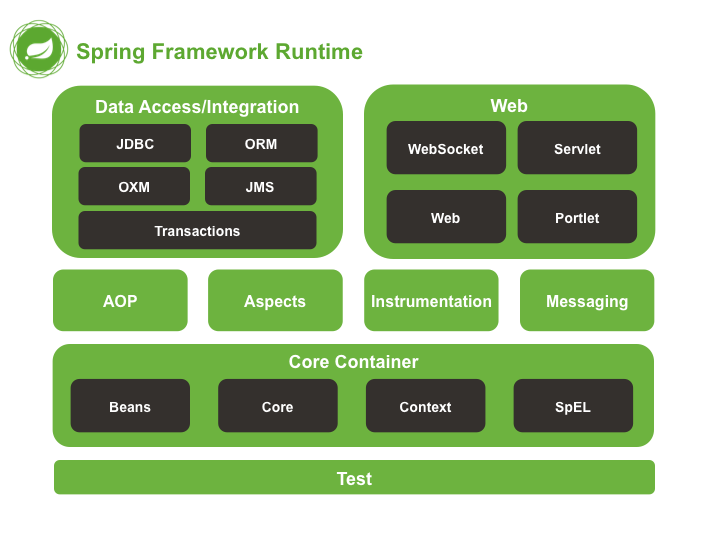
\includegraphics[width=0.95\textwidth]{images/spring-overview}
		\caption[Kontener Spring]{Kontener Spring wraz z modułami\\źródło: \cite{spring_documentation_reference}}
		\label{c3:information_level_figure}
	\end{figure}	
	 \textbf{Spring} składa się z ponad 20 samodzielnych modułów:
	 \begin{itemize}
	 	\item \textbf{Core Container} - fundament szkieletu na którym oparte są pozostałe modułu. Definiuje on funkcjonalność \textbf{Dependency Injection} oraz odwróconego sterowania, a także posiada definicję obiektów takich jak \textbf{Bean}, \textbf{Context}. Jego częścią są również klasy niezbędne do ładowania zasobów (plików), lokalizacji oraz \textbf{Expression Language}\footnote{Manipulowania obiektami poprzez wyrażania zapisane czystym tekstem, które są później tłumaczone na odpowiednie wywołania programowe},
	 	\item \textbf{Data Access/Integration} - określa sposób dostępu dla takich źródeł danych jak bazy danych, pliki XML, czy też zdalne źródła danych dostępne przez protokół JMS. Najważniejszą zaletą jest maksymalne wykorzystanie spójnych interfejsów do dostępu do danych i ukrycie ich źródła.  
	 	\item \textbf{Web} - składa się z klas, które pozwalają na inicjalizację kontenera odwróconego sterowania w kontekście działającego serwletu. Definiuje również funkcjonalność \textbf{Spring MVC}, które z kolei jest praktyczną implementacją wzorca \textbf{MVC},
	 	\item \textbf{AOP} - dostarcza sposoby oraz środki do programowania aspektowego.
	 \end{itemize}
	 Modularna budowa jest także praktyczną realizacją koncepcji odseparowania obszarów funkcjonalnych. Dzięki temu podejściu \textbf{Spring Framework} może być użyty w dowolnej konfiguracji, korzystając jedynie z wstrzykiwania zależności, odwróconego sterowania lub kolejnych modułów odpowiedzialnych za architekturę MVC dla aplikacji trójwarstwowych, dostępu do danych, komunikacji protokołem JMS czy też dynamicznego kontrolowania aplikacji poprzez protokół JMX. 
		
	\subsection{Użyte moduły Spring'a}
	
		\subsubsection{Spring MVC}
		\label{app:spring_mvc}
		\textbf{Spring MVC} jest zorganizowany wokół centralnego servletu \texbf{DispatcherServlet} oraz klas opatrzonych adnotacjami: \texbf{@Controller} lub \texbf{@RestController} - \textbf{kontrolerów}. Kontrolery są punktem łączącym warstwę widoku oraz logiki biznesowej. Konfigurowane za pomocą adnotacji są alternatywą dla standardowych serwletów. Ich główną zaletą jest możliwość ich wykorzystania w wielu przypadkach użycia, jako obiektów wywołujących operacje warstwy logiki biznesowej lub wspierających przetwarzanie danych z formularzy. Korzystając z takiego podejścia, programista nie jest zmuszony do definiowania kilku, bądź kilkunastu oddzielnych serwletów, z których każdy odpowiadałby innemu przypadkowi użycia lub pisania własnego silnika, który pozwalałby na generyczne i automatyczne wywołania konkretnych metod w zależności od adresu odpowiadającemu danemu kontrolerowi. 
		
		W warstwie kontrolerów wykorzystywany jest wysoce elastyczny mechanizm odpowiedzialny za konwertowanie danych między niekompatybilnymi typami. Dzięki niemu praktycznie nie istnieje konieczność tworzenia własnych mechanizmów przeznaczonych do tego celu. Ponadto wszelkie błędy związane z tym procesem nie są traktowane jako błędy systemu, ale jako błędy konwersji. Nie ma potrzeby redefiniowania modelu danych jako klas, których pola są prostymi typami danych, takimi jak liczby czy też łańcuchy znaków.
		
		Ostatecznie \textbf{Spring MVC} oferuje wsparcie dla operacji, której celem jest zrenderowanie pewnego widoku. Kontroler jest najczęściej odpowiedzialny za przygotowanie danych, które zostaną umieszczone w odpowiedzi wysłanej do klienta, oraz wybranie widoku poprzez unikatową nazwę. Dalszy proces zależy od wybranej technologii, użytej dla implementacji warstwy widoku. Istnieje możliwość wykorzystania zarówno plików JSP, jak i bibliotek gdzie końcowy widok jest złożeniem kilku innych. Z drugiej strony, kontroler nie jest ograniczony jedynie do wybrania widoków. Programista ma możliwość zwracania kompletnych kolekcji obiektów, które później zostaną wysłane do klienta w formacie JSON lub XML. Wybrany format może zostać łatwo zmieniony poprzez odpowiednią konfigurację projektu. 
		
		Głównymi zaletami \textbf{Spring MVC} są:
		\begin{itemize}
			\item wyraźny podział obowiązków pomiędzy poszczególnymi artefaktami (kontrolery, walidatory, formularze),
			\item uproszczona oraz wysoce elastyczna konfiguracja:
			\begin{itemize}
				\item adres pod którym kontroler jest dostępny,
				\item typ żądania: \textbf{GET}, \textbf{POST}, \textbf{DELETE}, \textbf{PUT},
				\item typ zwracanych danych: \textbf{nazwa widoku}, \textbf{JSON}, \textbf{XML},
			\end{itemize}
			\item brak konieczności duplikowania modelu danych,
			\item wsparcia dla różnorodnych technologi widoku: \textbf{JSP}, \textbf{Velocity}, \textbf{Apache Tiles} lub \textbf{JSF},
		\end{itemize}
		
		\subsubsection{Spring Data}
		\label{app:spring_data}
		Jest to praktyczne rozwiązanie problemu związanego z implementacją warstwy dostępu do danych. Eliminuje konieczność implementacji szablonowego i powtarzalnego kodu, którego głównym zadaniem jest wykonanie operacji na bazie danych określanych skrótem \textbf{CRUD}. Warto w tym miejscu zwrócić uwagę na generyczne API, które przekłada się na wysoki poziom abstrakcji, dzięki któremu możliwe jest korzystanie z praktycznie dowolnego źródła danych poprzez jednolity interfejs. Nie ważne staje się, czy dane przechowywane są w bazie danych \textbf{MySQL} lub \textbf{Oracle}, czy też w bazach nierelacyjnych, jak na przykład \textbf{MongoDB}. 
		
		\subsubsection{Spring Data JPA}
		\label{tech:spring_data_jpa}
		\textbf{Spring Data JPA} jest częścią \textbf{Spring Data}, zawierającym artefakty szczególnie użytecznie dla relacyjnych baz danych, jak na przykład MySQL. Jednym z tych elementów są repozytoria. Repozytorium jest niczym innym jak obiektem w naszej aplikacji dzięki któremu uzyskujemy faktyczny dostęp do danych i możemy nimi zarządzać. Co ważniejsze pojęcie to jest znacznie szersze niż mogłoby się wydawać, zwłaszcza w kontekście operacji wyszukiwania. Poniższy przykład kodu (listing \ref{tech:jpa_repo}) pokazuje klasę \textbf{JpaRepository}. Istniejące tam deklaracje metod są jedynie rozszerzeniem tych zdefiniowanych w kolejnych interfejsach: \textbf{PagingAndSortingRepository} oraz \textbf{CrudRepository}. Niemniej widać, że nawet na wyższym poziomie abstrakcji programiści \textbf{Spring Data} zadbali o bardzo wiele możliwych przypadków użycia, co przekłada się na końcową produktywność programisty. 
		\begin{code}
			\inputminted[
				linenos=true,
				fontfamily=monospace,
				obeytabs=true,
				samepage=true,
				fontsize=\scriptsize
			]{java}{codeSamples/jpa_repo.java}
			\caption[\textbf{JpaRepository}]{\textbf{JpaRepository} interfejs dla operacji bazodanowych na relacyjnej bazie danych w \textbf{Spring Data}}
			\label{tech:jpa_repo}
		\end{code}
		Ponadto nie ma konieczności implementacji takiego interfejsu. Aby utworzyć nowe repozytorium dla konkretnego obiektu domenowego należy utworzyć nowy interfejs. Zostanie on zaimplementowany podczas działania programu poprzez proxy. W tym miejscu proxy jest pośrednikiem, gdzie odbywa się proces tłumaczenia wywołań metod repozytorium na kwerendy SQL. Repozytoria posiadają także inną, bardzo interesującą cechę - automatyczne mapowanie metod na kwerendy. Jest to alternatywa dla nazywanych kwerend znanych ze standardu \textbf{JPA}. Zapytanie SQL pobierane jest z nazwy metody, co oczywiście wymusza pewną konwencję nazewnictwa. Niemniej jest to koncepcja ciekawa i idealnie nadaje się do tworzenia zapytań odnoszących się do 1 lub 2 atrybutów danego obiektu, których użycie jest równoznaczne z wykorzystaniem operatora \textbf{where} języka SQL. Wywołanie jest silnie typizowane, dlatego programista ma pewność, że obiekt będzie tego typu, który go interesuje. Dla bardziej skomplikowanych kwerend istnieje możliwość zadeklarowanie metody i oznaczenia jej adnotacją \textit{\@{}Query} z kodem JPQL \cite{jpql} \cite{spring_data}.
			
		Głównymi zaletami \textbf{Spring Data JPA} są:
		\begin{itemize}
			\item silne typizowanie danych,
			\item automatyczne tłumaczenie nazw metod na kwerendy SQL,
			\item szeroka gama operacji wyszukiwania,
			\item gotowa implementacja operacji \textbf{CRUD},
			\item uproszczona konfiguracja,
			\item jednolite interfejsy dostępu do danych, niezależne od źródła danych,
			\item minimalna ilość kodu niezbędna do utworzenia repozytoriów dla obiektów modelu danych
		\end{itemize}
		
		\subsubsection{Spring Security}	
		W momencie pisania aplikacji w technologii \textbf{Java EE}\footnote{Java Enterprise Editition} nie można zapomnieć o problemie nieautoryzowanego dostępu do strony lub do niektórych jej części. Sposób uzyskania takiej funkcjonalności jest zależny od kontenera w którym działamy. Inaczej to zagadnienie rozwiązywane jest w przypadku \textbf{Apache Tomcat}, a inaczej w przypadku \textbf{JBoss}. Oba z nich są serwerami aplikacji Javy, niemniej tak samo jak identyczny jest cel ich istnienia, tak samo różna jest implementacja kwestii autoryzacji. Dzięki \textbf{Spring Security} programista może korzystać z niezależnego od kontenera, wysoce konfigurowalnego mechanizmu kontroli dostępu do zasobów. W tym miejscu warto nadmienić, że moduł można dostosować do weryfikacji użytkowników zarówno z wykorzystaniem bazy danych, jak i stałej listy zawierającej nazwy użytkowników posiadających dostęp do aplikacji. Ponadto niewielkim nakładem pracy można dodać mechanizm kontroli, znany pod nazwą \textbf{Access Control List}. Jest to koncepcja, gdzie prawa dostępu (zarówno zapisu, odczytu czy tez modyfikacji) związane są z konkretnym typem obiektu. Wszystkie wyżej wymienione cechy czynią \textbf{Spring Security} doskonałym wyborem do ochrony wrażliwych elementów aplikacji internetowej. 
		
		\clearpage
		\subsubsection{Spring Web Flow}	
		\label{tech:spring_web_flow}
		\begin{quotation}
			``Przemieszczenia się kogoś, czegoś, przekazywanie, obieg czegoś.''\cite{polish_dictionary}
		\end{quotation}
		\textbf{SWF}\footnote{Skrót od Spring Web Flow} jest szczególnie użyteczne gdy aplikacja wymaga powtarzalności tych samych kroków w więcej niż jednym kontekście. Czasami taka sekwencja operacji jest częścią większego komponentu, co desygnuje je do wyodrębnienia ich jako samodzielnego modułu. Najlepszym przykładem użycia są w tym wypadku różnego rodzaju formularze służące do rejestracji użytkowników czy też kreatory nowych obiektów, gdzie umieszczenie wszystkich wymaganych pól na jednej stronie mogłoby zaciemnić obraz i uniemożliwić użytkownikowi zrozumienie działania. Ponieważ \textbf{SWF} jest modułem Spring, jest on w pełni zintegrowany z platformą \textbf{Spring MVC} \ref{app:spring_mvc} oraz silnikiem walidacji i konwersji typów.
		
		\textbf{Flow} \cite{spring_swf_reference} - jest centralnym obiektem modułu, w którym definiowane są kolejne kroki przepływu. Dzięki deklaratywnemu językowi XML definicje są czytelne, a możliwości których dostarcza \textbf{SWF} pozwala na kreowanie sekwencji w dowolny sposób, łączenie kroków z modelem danych, korzystania z podstawowych jak i zaawansowanych mechanizmów implementacji akcji. Akcje zawierają właściwą logikę biznesową dla konkretnej fazy przepływu, ale także pozwalają na pobieranie danych wejściowych oraz zwracanie wyników na ich podstawie. Są także zalecanym sposobem obsługi błędów związanych z logiką biznesową. 
		
		\begin{code}
			\inputminted[
				linenos=true,
				firstline=47,
				lastline=55,
				fontfamily=monospace,
				obeytabs=true,
				samepage=true,
				fontsize=\scriptsize
			]{xml}{../SpringAtom_thesis/src/main/webapp/ui/wizard/NewReportWizard/flow.xml}
			\caption[Deklaratywna deklaracja stanu - kroku dla przepływu w rozumieniu \textbf{Spring Web Flow}]{
				Deklaratywna deklaracja stanu - kroku dla przepływu w rozumieniu \textbf{Spring Web Flow}, źródło: opracowanie własne			
			}
			\label{app:swf_view_state}
		\end{code}
		
		Przykład \ref{app:swf_view_state} pokazuje kod XML, który definiuje jeden z kroków - stanów. Powyższy przykład korzysta z klasy \begin{code}org.springframework.webflow.action.FormAction\end{code}. Metoda \begin{code}setupForm\end{code} może służyć między innymi do wprowadzenia danych wejściowych do kontekstu przepływu.
		\begin{code}
			\inputminted[
				linenos=true,
				firstline=69,
				lastline=76,
				fontfamily=monospace,
				obeytabs=true,
				samepage=true,
				fontsize=\scriptsize
			]{java}{../SpringAtom_thesis/src/main/java/org/agatom/springatom/web/flows/wizards/wizard/rbuilder/PickEntityFormAction.java}
			% src file used
			\caption[Metoda \textit{setupForm} dla \textbf{Spring Web Flow}]{\textit{setupForm} - metoda
				\textit{setupForm} wykorzystywana w definicji kroku \ref{app:swf_view_state} do umieszczenia danych w kontekście
				przepływu, źródło: opracowanie własne
			}
			\label{app:swf_setupForm}
		\end{code}
